\section{ROS (Robot Operating System)}
\subsection{ROSとは}
ROS(Robot Operating System)とはOpen Source Robotics Foundationによって管理されているソフトウェア開発者のロボット・アプリケーション作成を支援するフレームワークである.
具体的には,ハードウェア抽象化,デバイスドライバ,ライブラリ,視覚化ツール,メッセージ通信,パッケージ管理などが提供されている.
つまりROSは汎用コンピュータ向けのOSではなく,汎用コンピュータ向けOS上で動作するメタOSとして捉えることができる\cite{kurazume}.

\refig{ros_topic}に示すようにROSではプロセス(実行プログラム)はノードという単位で扱い,ノード間の通信はトピックと呼ばれる``Publisher/Subscriber''モデルで実現される\cite{ogura}.

これにより,プログラミング言語や通信相手さえ意識することなく簡単にプロセス間通信を実現できる.
これは各ノード間のインタフェース,即ちトピックの名前と型さえ決定すればノードごとに独立して開発を行うことができるという利点でもある.\\

以上の利点を鑑み,本研究室ではROSがインストール可能なマイコンボードであるRaspberryPi3 Model B上にROSをインストールして開発を進めていくこととした.

\begin{figure}[htb]
  \centering
    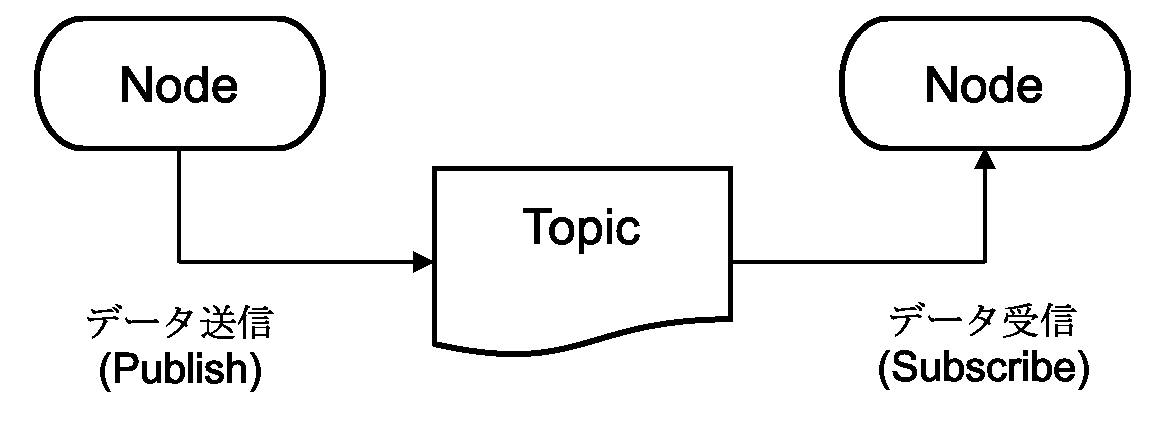
\includegraphics[width=0.5\hsize]{picture/eps/ros_topic.eps}
    \caption{ROSノードとトピックの概念}
    \label{fig::ros_topic}
\end{figure}



\begin{figure}[htb]
  \centering
    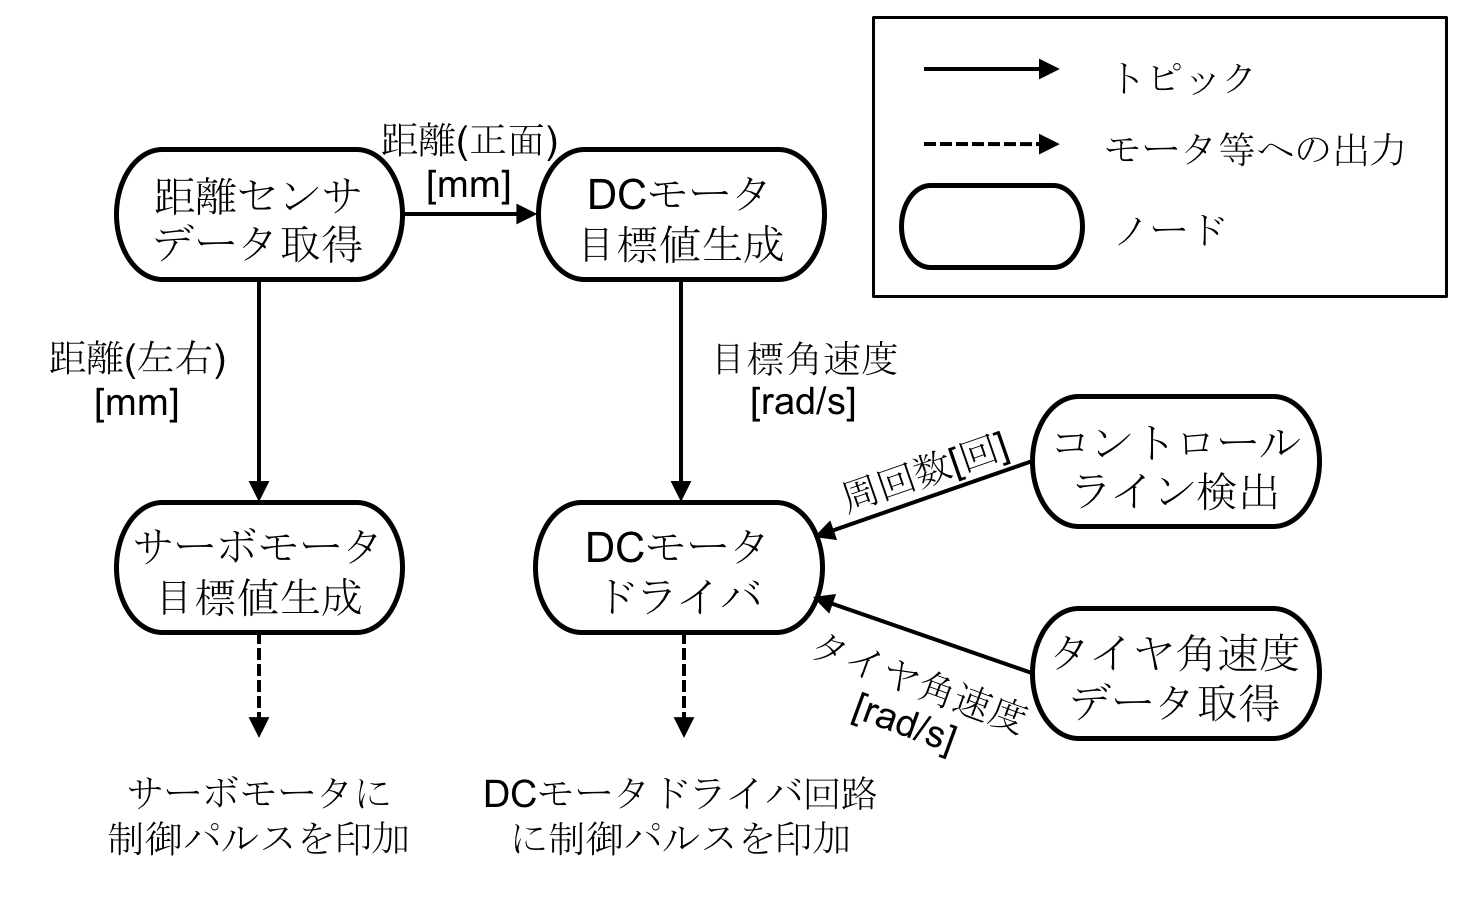
\includegraphics[width=0.8\hsize]{picture/eps/ros_nodes.eps}
    \caption{ROSノードとトピックの構成}
    \label{fig::ros_nodes}
\end{figure}

\newpage
\subsection{ROSノードとトピックの構成}
\refig{ros_nodes}に開発するROSノードとトピックの構成を示す.各ノードの役割は次の通りである.
\begin{description}

    \item[距離センサデータ取得] \mbox{} \\
      機体前方及び両側面に設置した距離センサからシリアルバス規格の一つである$\mathrm{I^2C}$を介して距離データを$\mathrm{[mm]}$単位で取得し外れ値処理や正規化を施した後にPublishする.
    \item[コントロールライン検出] \mbox{} \\
      機体後方下部に設置したフォトリフレクタによってコントロールラインを通過した回数をカウントしPublishする.

    \item[タイヤ角速度データ取得] \mbox{} \\
      回転方向は考慮しないため,ロータリーエンコーダのA相のパルスのみをカウントし,ロータリーエンコーダの一周あたりの出力パルス数$(500パルス)$,サンプリング周期$(0.01\unit{s})$,ロータリーエンコーダの軸に取り付けたピニオンギアとドライブシャフトに取り付けたギア間のギア比$(2.74)$を考慮して$k$時点のタイヤの角速度$\omega(k)$を$\unit{rad/s}$単位で算出する.また,ノイズ対策として算出した角速度を\refeq{lpf}で表されるデジタルフィルタ(LPFに相当)に通した結果をPublishするようにしている.ただし,$\alpha$は$0〜1$の範囲で定める定数である.\\
      \begin{equation}
      	\omega(k)=\alpha\omega(k)+(1-\alpha)\omega(k-1)\label{eq::lpf}
      \end{equation}

    \item[DCモータ目標値生成] \mbox{} \\
      機体前方方向の距離データをSubscribeし,それをもとにDCモータに与える目標値を生成しPublishする.

    \item[DCモータドライバ] \mbox{} \\
      DCモータに与える目標値とタイヤの角速度データをSubscribeし,PI制御則に基づきDCモータを駆動する.

    \item[サーボモータ目標値生成] \mbox{} \\
      機体前方の距離データをSubscribeし,それをもとにサーボモータに与える目標値を生成しその後直接サーボモータを駆動する.サーボモータドライバノードが存在しないのはサーボモータの軸にロータリーエンコーダがついておらず角度フィードバックが出来ないためである.

  \end{description}
